
\chapter{Linear Analysis of Numerical Methods}
\label{chp:AnalNumMethod}
An important property of a numerical method is convergence. Convergence guarantees that as we increase the spatial and temporal resolution of a numerical method, its numerical solution approaches the solution of the partial differential equations. For linear partial differential equations the Lax-equivalence theorem states that a numerical method is convergent if and only if it is stable and consistent \cite{Lax-Richtmyer-1956-267}. A numerical scheme is consistent if the error introduced by the numerical method over a time step approaches zero as the spatial and temporal resolution is increased. While stability means that the errors from previous time steps are not amplified by the current time step.

Another important property of a numerical method modelling dispersive wave equations such as the Serre equations is its dispersion relation. The dispersion properties of a numerical method determine the phase and group velocity of travelling waves in its numerical solutions. Because the Serre equations possess dispersion properties that well approximate those of linear theory for water waves [], approximating the dispersion properties of the Serre equations well by the numerical method is essential.

We analysed the convergence and the dispersion properties of our numerical methods for the linearised Serre equations with horizontal beds. To offer some insight into the convergence properties of our numerical method for the full Serre equations and because the dispersion properties are derived from the linearised Serre equations. 

The analysis of the convergence and dispersion properties of our numerical methods rely on establishing a relation of the form

\begin{equation}
\label{eqn:linearanalaim}
\begin{bmatrix}
h \\G
\end{bmatrix}^{n+1}_j = \matr{E} \begin{bmatrix}
h \\G
\end{bmatrix}^{n}_j
\end{equation}
 where $\matr{E}$ is the evolution matrix relating the conserved quantities $h$ and $G$ at time level $t^n$ with the conserved quantities at time level $t^{n+1}$. The evolution matrix $\matr{E}$ is obtained in the analyses by propagating Fourier modes through the numerical scheme. 
 
 We begin our analyses by giving the linearised Serre equations with horizontal beds. We then derive $\matr{E}$ \eqref{eqn:linearanalaim} for the second-order FEVM and perform the convergence and dispersion analysis. We will then present the results of these analyses for all numerical methods and the unique steps required to perform the analyses for the other numerical methods.
 

 
\section{Linearised Serre equations with horizontal bed}
The Serre equations with a horizontal bed \eqref{eqn:FullSerreNonConHorizbed} are linearised by considering waves as small perturbations $\delta\eta$ and $\delta\upsilon$ on a flow with a mean height $H$ and a mean velocity $U$ respectively. So we have
\begin{subequations}
	\label{eq:pertubation}
\begin{align}
h(x,t) &= H + \delta \eta(x,t) + \mathcal{O}\left(\delta^2 \right), \\
u(x,t) &= U + \delta \upsilon(x,t) + \mathcal{O}\left(\delta^2 \right),
\end{align}
\end{subequations}
where $\delta \ll 1$. These waves are relatively small so terms of order $\delta^2$ are negligible. We substitute \eqref{eq:pertubation} into the Serre equations and neglect terms of order $\delta^2$ to obtain

\begin{subequations}
	\begin{gather}
		\label{eqn:LinCont}
		\frac{\partial  \left(\delta\eta \right)}{\partial  t} + H\frac{\partial  \left(\delta\upsilon \right)}{\partial  x} + U\frac{\partial  \left(\delta\eta \right)}{\partial  x}  = 0,
	\end{gather}
	\begin{gather}
	\label{eqn:LineMome}
	H\frac{\partial  \left(\delta\upsilon \right)}{\partial  t} + gH\frac{\partial  \left(\delta\eta \right)}{\partial  x} + UH\frac{\partial  \left(\delta\upsilon \right)}{\partial  x} - \frac{H^3}{3}\left(U\frac{\partial^3  \left(\delta\upsilon \right)}{\partial  x^3} + \frac{\partial^3  \left(\delta\upsilon \right)}{\partial  x^2 \partial  t}  \right)  = 0
	\end{gather}
\label{eqn:LinSerre}	
and for $G$
\begin{gather}
	G = UH + U \delta \eta + H \delta \upsilon -\frac{H^3}{3} \frac{\partial^2 \left(\delta\upsilon \right)}{\partial x^2}.
	\label{eqn:LinConSerre}
\end{gather}	
\end{subequations}
The these equations can be reformulated  into conservation law form
\begin{subequations}
	\begin{gather}
	\label{eqn:LinContG}
	\frac{\partial  \eta}{\partial  t} +\frac{\partial}{\partial  x} \left(H\upsilon + U \eta\right) = 0,
	\end{gather}
	\begin{gather}
	\label{eqn:LineMomeG}
	\frac{\partial  G}{\partial  t} + \frac{\partial}{\partial  x}\left(UG + UH\upsilon + gH \eta\right) = 0.
	\end{gather}
	and for $G$
	\begin{gather}
	G = UH + U \eta + H \upsilon -\frac{H^3}{3} \frac{\partial^2 \left(\upsilon \right)}{\partial x^2}.
	\label{eqn:LinConSerreG}
	\end{gather}
	\label{eqn:LinSerreG}	
\end{subequations}
We have absorbed the $\delta$ factor into the corresponding $\eta$ and $\upsilon$ terms to simplify the notation.

\section{Evolution Matrix}
To derive the evolution matrix we first assume that the solutions of the linearised Serre equations with horizontal beds \eqref{eqn:LinSerreG} are periodic in space and time. In particular, we assume that $\eta$ and $\upsilon$ are Fourier modes, which for a general quantity $q$ means
\begin{equation}
q(x,t) = q(0,0) e^{i\left(\omega t + kx\right)}.
\label{eqn:FourierNode}
\end{equation}
This is precisely the assumption made to derive the analytical dispersion relation of the linearised Serre equations []. A consequence of a quantity $q$ being a Fourier mode represented on uniform temporal and spatial grid is that for any real numbers $m$ and $l$ we have
\begin{equation}
q^{n + m}_{j + l} = q^n_j e^{ i \left(m \omega \Delta t + l k \Delta x\right)}.
\label{eqn:fourierfactor}
\end{equation}
Because $\eta$ and $\upsilon$ are Fourier modes then so is $G$. Furthermore, the cell averages of these quantities $\overline{\eta}$, $\overline{\upsilon}$ and $\overline{G}$ are Fourier modes as well.

\subsection{Overview of the analysis}
We will now present a brief overview of the analysis for a single evolution step of the second-order FEVM. Given the vectors of the cell averages $\overline{\vecn{\eta}}$ and $\overline{\vecn{G}}$ at the current time the second-order FEVM evolution step progresses in the following way
\begin{enumerate}
	\item Reconstruction: We use the operator $\mathcal{M}$ to calculate $\eta$ and $G$ at the cell midpoint $x_{j}$ from the cell averages. We also reconstruct $\eta$ and $G$ at the cell interface $x^-_{j+1/2}$ and $x^+_{j+1/2}$ from the cell average values using $\mathcal{R}^{-}$ and $\mathcal{R}^{+}$ respectively. So that
	\begin{align*}	&\eta_j = \mathcal{M}\left(\overline{\vecn{\eta}}\right),& G_j = \mathcal{M}\left(\overline{\vecn{G}}\right),\\
	&\eta^-_{j+1/2} = \mathcal{R}^{-}\left(\overline{\vecn{\eta}}\right),  &G^-_{j+1/2} = \mathcal{R}^{-}\left(\overline{\vecn{G}}\right), \\
	&\eta^+_{j+1/2} = \mathcal{R}^{+}\left(\overline{\vecn{\eta}}\right),  &G^+_{j+1/2} = \mathcal{R}^{+}\left(\overline{\vecn{G}}\right). \\	
	\end{align*}
	\item Calculate $\upsilon$: We use the map $\mathcal{G}$ given by the elliptic equation between $G$ and $\upsilon$ to calculate $\upsilon_{j+1/2} $ from ${\vecn{G}}$ and $H$
	\[\upsilon_{j+1/2} = \mathcal{G}\left(H, {\vecn{G}}\right).\]
	\item Calculate Flux: We calculate the average flux across the cell boundary $x_{j+1/2}$ over time; $F_{j+1/2}$ using $\mathcal{F}$
	\[F_{j+1/2} =\mathcal{F} \left(\eta^-_{j+1/2}, G^-_{j+1/2},\eta^+_{j+1/2}, G^+_{j+1/2},\upsilon_{j+1/2}  \right). \]
	\item Forward Euler Step: We repeat this process for each cell edge and then apply the update formula \eqref{eqn:evolupdatescheme} to update the vectors $\overline{\vecn{\eta}}$ and $\overline{\vecn{G}}$ from the current time level to the next time level with first-order accuracy in time.
	\item SSP Runge-Kutta Steps: We repeat the Euler step encapsulated by steps 1-4 and use SSP Runge-Kutta time stepping [] to calculate $\overline{\vecn{\eta}}$ and $\overline{\vecn{G}}$ at the next time level with second-order accuracy in time.
\end{enumerate}

We will now derive expressions for all the operators in the evolution step, which will be linear due to our assumption that $\eta$ and $\upsilon$ are Fourier modes. We will then combine these to derive $\matr{E}$ for the second-order FEVM.

\subsection{1. Reconstruction}
Given $\overline{\vecn{\eta}}$ and $\overline{\vecn{G}}$ at $t^n$ the second step of our numerical method is to calculate $\eta$ and $G$ at $x_j$ using $\mathcal{M}$ and at $x^-_{j+1/2}$ and $x^+_{j+1/2}$ using $\mathcal{R}^-$ and $\mathcal{R}^+$ respectively. The derivation of these operators is given in terms of a general quantity $q$, as they are the same for $\eta$ and $G$.
\subsubsection{Cell average values to nodal values: $\mathcal{M}$}
For the second-order FEVM we use the fact that
\begin{equation*}
\overline{q}_j =q_j  + \mathcal{O}\left(\Delta x^2\right).
\end{equation*}
%
So to attain second-order accuracy we use
%
\begin{equation}
\label{eqn:Mfactorfourier}
q_j = \overline{q}_j  = \mathcal{M} \overline{q}_j.
\end{equation}
Therefore, we have a factor $\mathcal{M}=1$ representing the map between cell averages and nodal values for our numerical method.

\subsubsection{Cell average values to interface values: $\mathcal{R}^-$ and $\mathcal{R}^+$}

We reconstruct $\eta$ and $G$ at $x^-_{j+1/2}$ and $x^+_{j+1/2}$. These quantities can be discontinuous across the cell interfaces in our finite volume method. However, since we are assuming that these quantities are Fourier modes and therefore smooth we do not require non-linear limiters to ensure our scheme is TVD. Without limiters our reconstruction scheme for $\eta$ and $G$ can be written for a general quantity $q$ as

\begin{equation*}
q^-_{j+\frac{1}{2}} = \overline{q}_j + \frac{- \overline{q}_{j - 1} + \overline{q}_{j+ 1} }{4},
\end{equation*}
\begin{equation*}
q^+_{j+\frac{1}{2}} = \overline{q}_{j+1} + \frac{- \overline{q}_{j} + \overline{q}_{j+ 2}}{4}.
\end{equation*}

Using \eqref{eqn:fourierfactor} and \eqref{eqn:Mfactorfourier} these equations become

\begin{subequations}
	\label{eqn:RpmfactorFDVM}
	\begin{align}
	&q^-_{j+\frac{1}{2}} =\overline{q}_j + \frac{- \overline{q}_{j} e^{-ik\Delta x} + \overline{q}_{j} e^{ik\Delta x}}{4} = \left(1  + \frac{i\sin\left(k\Delta x\right)}{2} \right)\overline{q}_{j} =\mathcal{R}^- \overline{q}_{j},\\
	&q^+_{j+\frac{1}{2}}= \frac{\overline{q}_{j}e^{ik\Delta x} + \overline{q}_{j} + \overline{q}_{j}e^{2ik\Delta x} }{4} = e^{ik\Delta x}\left(1  - \frac{i\sin\left(k\Delta x\right)}{2} \right)\overline{q}_{j} = \mathcal{R}^+ \overline{q}_{j}.
	\end{align}
\end{subequations}
These are the reconstruction factors for both $\eta^{\pm}_{j+1/2}$ and $G^{\pm}_{j+1/2}$.

\subsection{2. Calculate $\upsilon$}
We begin our FEM for \eqref{eqn:LinConSerreGu0} with its weak formulation, obtained by multiplying \eqref{eqn:LinConSerreGu0} by a test function $\tau$ and integrating over the domain $\Omega$
\begin{equation*}
\int_{\Omega}G \tau \; dx = UH\int_{\Omega} \tau \; dx + U \int_{\Omega} \eta \tau \; dx +   H\int_{\Omega} \upsilon \tau \; dx  + \frac{H^3}{3} \int_{\Omega} \frac{\partial \upsilon}{\partial x } \frac{\partial \tau}{\partial x }\; dx.
\end{equation*}
For $G$ we use the basis functions $\psi^+_{j - 1/2}$ and $\psi^-_{j + 1/2}$ defined in Chapter [], which means $G$ is linear inside a cell with discontinuous jumps at the cell edges. For $\tau$ and $\upsilon$ we use the basis functions $\phi_{j-1/2}$, $\phi_{j}$ and $\phi_{j+1/2}$ defined in Chapter [], so that $\tau$ and $\upsilon$ are quadratic functions inside a cell that are continuous across the cell edges. Substituting in the approximations to our quantities based on these basis functions and breaking our integration up into the sum of the integrals over a cell as we did in Chapter [], we get that

\begin{multline*}
\sum_j \int_{x_{j-1/2}}^{x_{j + 1/2}} \left(G^+_{j-1/2}\psi^+_{j - 1/2} + G^-_{j+1/2}\psi^-_{j + 1/2}\right) \begin{bmatrix}
\phi_{j-1/2}\\\phi_j \\\phi_{j+1/2}
\end{bmatrix}  \; dx= \\ \sum_j UH\int_{x_{j-1/2}}^{x_{j + 1/2}}  \begin{bmatrix}
\phi_{j-1/2}\\\phi_j \\\phi_{j+1/2}
\end{bmatrix}  \; dx + \sum_j U\int_{x_{j-1/2}}^{x_{j + 1/2}} \left(\eta^+_{j-1/2}\psi^+_{j - 1/2} + \eta^-_{j+1/2}\psi^-_{j + 1/2}\right) \begin{bmatrix}
\phi_{j-1/2}\\\phi_j \\\phi_{j+1/2}
\end{bmatrix}  \; dx \\ \\   +\sum_j H\int_{x_{j-1/2}}^{x_{j + 1/2}} \left(\upsilon_{j-1/2}\phi_{j - 1/2} + \upsilon_{j}\phi_{j}+ \upsilon_{j+1/2}\phi_{j + 1/2}\right) \begin{bmatrix}
\phi_{j-1/2}\\\phi_j \\\phi_{j+1/2}
\end{bmatrix}  \; dx \\ + 
\sum_j \frac{H^3}{3}\int_{x_{j-1/2}}^{x_{j + 1/2}} \left(\upsilon_{j-1/2} \frac{\partial \phi_{j - 1/2} }{\partial x} + \upsilon_{j}\frac{\partial \phi_{j} }{\partial x}+ \upsilon_{j+1/2}\frac{\partial \phi_{j + 1/2} }{\partial x}\right) \begin{bmatrix}
\dfrac{\partial \phi_{j - 1/2} }{\partial x}\\ \\\dfrac{\partial \phi_{j} }{\partial x}\\ \\\dfrac{\partial \phi_{j + 1/2} }{\partial x}   \end{bmatrix} \; dx.
\end{multline*}
Calculating all the integrals of the appropriate basis function combinations we get 
\begin{multline*}
\sum_j \frac{\Delta x}{6}\begin{bmatrix} G^+_{j -1/2} \\2 G^+_{j -1/2}+2 G^-_{j +1/2} \\ G^-_{j +1/2} \end{bmatrix} = \sum_jUH \frac{\Delta x}{6}\begin{bmatrix} 1 \\4 \\ 1 \end{bmatrix} +  \sum_j \frac{\Delta x}{6}U\begin{bmatrix} \eta^+_{j -1/2} \\2 \eta^+_{j -1/2}+2 \eta^-_{j +1/2} \\ \eta^-_{j +1/2} \end{bmatrix}\\ + \sum_j \left(H\frac{\Delta x}{30}\begin{bmatrix} 4 &2 &-1 \\2 &16 &2  \\-1 &2 &4 \end{bmatrix} + \frac{H^3 }{9\Delta x}\begin{bmatrix} 7 &-8 &1  \\-8 &16 &-8  \\1 &-8 &7  \end{bmatrix} \right) \begin{bmatrix} \upsilon_{j -1/2} \\\upsilon_{j} \\ \upsilon_{j +1/2} \end{bmatrix}.
\end{multline*} 
%minmod limiter for G
Using \eqref{eqn:fourierfactor} and the reconstructions $\mathcal{R}^+$ and $\mathcal{R}^-$ used on $\overline{G}$ to obtain $G^+_{j +1/2}$ and $G^-_{j +1/2}$ respectively \eqref{eqn:RpmfactorFDVM}, we obtain

\begin{multline*}
\sum_j \frac{\Delta x}{6} \begin{bmatrix} e^{-ik\Delta x} \mathcal{R}^+ \overline{G}_{j} \\2 e^{-ik\Delta x} \mathcal{R}^+\overline{G}_{j} +2 \mathcal{R}^- \overline{G}_{j}\\ \mathcal{R}^- \overline{G}_{j} \end{bmatrix} =   \sum_jUH \frac{\Delta x}{6}\begin{bmatrix} 1 \\4 \\ 1 \end{bmatrix} +  \sum_j \frac{\Delta x}{6} U \begin{bmatrix} e^{-ik\Delta x} \mathcal{R}^+ \overline{\eta}_{j} \\2 e^{-ik\Delta x} \mathcal{R}^+\overline{\eta}_{j} +2 \mathcal{R}^- \overline{\eta}_{j}\\ \mathcal{R}^- \overline{\eta}_{j} \end{bmatrix}  \\\sum_j \left(H\frac{\Delta x}{30}\begin{bmatrix} 4 &2 &-1 \\2 &16 &2  \\-1 &2 &4 \end{bmatrix} + \frac{H^3 }{9\Delta x}\begin{bmatrix} 7 &-8 &1  \\-8 &16 &-8  \\1 &-8 &7  \end{bmatrix} \right) \begin{bmatrix} e^{-ik\frac{\Delta x}{2}}\upsilon_{j} \\\upsilon_{j} \\ e^{ik\frac{\Delta x}{2}}\upsilon_{j} \end{bmatrix}
\end{multline*}
\begin{multline*}
\sum_j \frac{\Delta x}{6}\begin{bmatrix} e^{-ik\Delta x} \mathcal{R}^+ \\2 e^{-ik\Delta x} \mathcal{R}^+ +2 \mathcal{R}^-\\ \mathcal{R}^- \end{bmatrix} \overline{G}_{j} = \sum_jUH \frac{\Delta x}{6}\begin{bmatrix} 1 \\4 \\ 1 \end{bmatrix} +  \sum_j \frac{\Delta x}{6}\begin{bmatrix} e^{-ik\Delta x} \mathcal{R}^+ \\2 e^{-ik\Delta x} \mathcal{R}^+ +2 \mathcal{R}^-\\ \mathcal{R}^- \end{bmatrix} \overline{\eta}_{j} \\ + \sum_j \Bigg(H\frac{\Delta x}{30}\begin{bmatrix} 4e^{-ik\frac{\Delta x}{2}} +  2 - e^{ik\frac{\Delta x}{2}}\\2e^{-ik\frac{\Delta x}{2}}  + 16  +2 e^{ik\frac{\Delta x}{2}}  \\ -e^{-ik\frac{\Delta x}{2}} +  2 + 4e^{ik\frac{\Delta x}{2}} \end{bmatrix} \\+ \frac{H^3 }{9\Delta x}\begin{bmatrix} 7e^{-ik\frac{\Delta x}{2}} -8 + e^{ik\frac{\Delta x}{2}} \\ -8e^{-ik\frac{\Delta x}{2}} +  16  -8e^{ik\frac{\Delta x}{2}} \\ e^{-ik\frac{\Delta x}{2}} -8 + 7e^{ik\frac{\Delta x}{2}} \end{bmatrix}  \Bigg) \upsilon_j.
\end{multline*}
These vectors represent three equations for the $j^{th}$ cell, the first relates $\overline{G}_j$ to $\upsilon_{j-1/2}$, the second relates $\overline{G}_j$ to $\upsilon_{j}$ and the third relates $\overline{G}_j$ to $\upsilon_{j+1/2}$. Since the flux calculation \eqref{eqn:etafluxapprox} only requires $\upsilon_{j+1/2}$ we will neglect the other equations here. So far we have only given the equation for $\upsilon_{j+1/2}$ from the $j$th cell, but $\upsilon_{j+1/2}$ will also have an equation for the $(j+1)$th cell as $\phi_{j+1/2}$ is non-zero there. Taking this into account we get that the  third equation is
\begin{multline*}
\frac{\Delta x}{6} \left(\mathcal{R}^- + \mathcal{R}^+ \right)\overline{G}_{j} = \frac{\Delta x}{6} 2UH   + \frac{\Delta x}{6} U \left(\mathcal{R}^- + \mathcal{R}^+ \right)\overline{\eta}_{j} \\ \Bigg(H\frac{\Delta x}{30} \left( -e^{-ik\frac{\Delta x}{2}} +  2 + 4e^{ik\frac{\Delta x}{2}} + e^{ik{\Delta x}}\left(4e^{-ik\frac{\Delta x}{2}} +  2 - e^{ik\frac{\Delta x}{2}}\right) \right)  \\+ \frac{H^3 }{9\Delta x} \left(  e^{-ik\frac{\Delta x}{2}} -8 + 7e^{ik\frac{\Delta x}{2}}  + e^{ik{\Delta x}}\left(7e^{-ik\frac{\Delta x}{2}} -8 + e^{ik\frac{\Delta x}{2}}  \right)  \right)   \Bigg) \upsilon_j.
\\ = \frac{\Delta x}{3}UH   + \frac{\Delta x}{6} U \left(\mathcal{R}^- + \mathcal{R}^+ \right)\overline{\eta}_{j} +  \Bigg[H\frac{\Delta x}{30} \left( 4\cos\left(\frac{k \Delta x}{2}\right) - 2\cos\left({k \Delta x}\right) + 8\right)   \\+ \frac{H^3 }{9\Delta x} \left(-16\cos\left(\frac{k\Delta x}{2}\right) + 2 \cos\left(k \Delta x\right) + 14\right) \Bigg]e^{i k \frac{\Delta x}{2}} \upsilon_{j}.
\end{multline*}
Since $e^{i k \frac{\Delta x}{2}} \upsilon_{j} =  \upsilon_{j+1/2}$ \eqref{eqn:fourierfactor} we have that
\begin{multline}
\label{eqn:2ndFEMutoG}
\upsilon_{j+1/2} =  \left[\left(\frac{\Delta x}{6} \left(\mathcal{R}^- + \mathcal{R}^+ \right)\right)  \overline{G}_{j}  - \frac{\Delta x}{3}UH - U\left(\frac{\Delta x}{6} \left(\mathcal{R}^- + \mathcal{R}^+ \right)\right)  \overline{\eta}_{j}   \right]\\
\div  \Bigg[H\frac{\Delta x}{30} \left( 2\left(2\cos\left(\frac{k \Delta x}{2}\right) - \cos\left({k \Delta x}\right) + 4\right)  \right)  \\+ \frac{H^3 }{9\Delta x}\left(-16\cos\left(\frac{k\Delta x}{2}\right) + 2 \cos\left(k \Delta x\right) + 14\right)    \Bigg]
\\= \mathcal{G}^G \overline{G}_{j} + \mathcal{G}^{\eta} \overline{\eta}_{j} + \mathcal{G}^c .
\end{multline}
 

\subsection{3. Flux calculation}
To calculate the average flux $F_{j+1/2}$ we use Kurganov's method \cite{Kurganov-etal-2001-707}. For the linearised Serre equations we have the wave speed bounds \eqref{eqn:WaveVelocitiesBound}, so that
\begin{align}
a^-_{j+ 1/2} = \min \left\lbrace 0,  U - \sqrt{g H} \right \rbrace& &\text{and}& &a^+_{j+ 1/2} =  \max \left\lbrace 0, U + \sqrt{g H} \right \rbrace .
\label{eqn:wavespeedboundslinSerre}
\end{align}

Therefore our method has three possibilities depending on $U$, $g$ and $H$;  supercritical flow to the left $U < - \sqrt{gH}$, subcritical flow $-\sqrt{gH} \le U \le \sqrt{gH}$ and supercritical flow to the right $\sqrt{gH} < U$. We will derive the flux operators for each of these scenario separately.

\subsubsection{Left supercritical flow $U < - \sqrt{gH}$:}
For left supercritical flow; $U < - \sqrt{gH}$  we have that from \eqref{eqn:wavespeedboundslinSerre} that $a^-_{j+ 1/2} = U - \sqrt{g H}$ and $a^+_{j+ 1/2} =  0$. For these values the Kurganov flux approximation for a general quantity $q$ [] reduces to 
\begin{equation}
F_{j+\frac{1}{2}} = f\left(q^+_{j+\frac{1}{2}}\right)
\label{eqn:fluxleftsupercrit}
\end{equation}

Substituting our flux function for $\eta$ \eqref{eqn:LinContG} into our Kurganov flux approximation \eqref{eqn:fluxleftsupercrit} we obtain
\begin{equation*}
F^\eta_{j+\frac{1}{2}} = H \upsilon_{j+1/2} + U \eta^+_{j+1/2}
\end{equation*}
since $\upsilon$ is continuous and therefore $\upsilon_{j+1/2} = \upsilon_{j+1/2}^+ = \upsilon_{j+1/2}^- $. Using our solver for $\upsilon$ \eqref{eqn:2ndFEMutoG} and the reconstruction \eqref{eqn:RpmfactorFDVM} we have
\begin{align}
F^\eta_{j+\frac{1}{2}} &= H \left(\mathcal{G}^G \overline{G}_{j} + \mathcal{G}^{\eta} \overline{\eta}_{j} + \mathcal{G}^c\right) + U \eta^+_{j+1/2} \nonumber \\ &= \left(H \mathcal{G}^{\eta} + U \mathcal{R}^+ \right)  \overline{\eta}_{j} + H \mathcal{G}^G \overline{G}_{j} + H\mathcal{G}^c \nonumber \\
&= F^{\eta, \eta}_{j+\frac{1}{2}} \overline{\eta}_{j} + F^{\eta, G}_{j+\frac{1}{2}} \overline{G}_{j} + F^{\eta, c}_{j+\frac{1}{2}}
\label{eqn:Fluxfactorsupercritetaleft}
\end{align}

Substituting our flux function for $G$ \eqref{eqn:LineMomeG} into our Kurganov flux approximation \eqref{eqn:fluxleftsupercrit} we obtain
\begin{equation*}
F^G_{j+\frac{1}{2}} =U G^+_{j+1/2} + U  H \upsilon_{j+1/2} + gH \eta^+_{j+1/2}
\end{equation*}
Using our elliptic solver \eqref{eqn:2ndFEMutoG} and our interface reconstruction \eqref{eqn:RpmfactorFDVM} we have
\begin{align}
F^G_{j+\frac{1}{2}} &=  U G^+_{j+1/2} + UH \left(\mathcal{G}^G \overline{G}_{j} + \mathcal{G}^{\eta} \overline{\eta}_{j} + \mathcal{G}^c\right) + gH \eta^+_{j+1/2} \nonumber \\ &= \left(UH \mathcal{G}^{\eta} + gH \mathcal{R}^+ \right)  \overline{\eta}_{j} + \left(U\mathcal{R}^+  +  UH \mathcal{G}^G \right) \overline{G}_{j} + UH\mathcal{G}^c \nonumber \\
&= F^{G, \eta}_{j+\frac{1}{2}} \overline{\eta}_{j} + F^{G, G}_{j+\frac{1}{2}} \overline{G}_{j} + F^{G, c}_{j+\frac{1}{2}}
\label{eqn:FluxfactorsupercritGleft}
\end{align}


\subsubsection{Subcritical flow $-\sqrt{gH} \le U \le \sqrt{gH}$:}
When the flow is subcritical we have $-\sqrt{gH} \le U \le \sqrt{gH}$, which means that $a^-_{j+ 1/2} = U - \sqrt{g H}$ and $a^+_{j+ 1/2} =  U + \sqrt{g H}$. So our Kurganov flux approximation for a general quantity $q$ [] reduces to

\begin{align}
F_{j+\frac{1}{2}} = &\frac{U}{2 \sqrt{gH}} \left[f\left(q^-_{j+\frac{1}{2}}\right) - f\left(q^+_{j+\frac{1}{2}}\right) \right]  + \frac{1}{2}\left[f\left(q^-_{j+\frac{1}{2}}\right) + f\left(q^+_{j+\frac{1}{2}}\right)\right] \nonumber \\ &+ \dfrac{U^2 - gH}{2\sqrt{g H}} \left [ q^+_{j+\frac{1}{2}} - q^-_{j+\frac{1}{2}} \right ].
\label{eqn:fluxsubcrit}
\end{align}

Substituting in the flux function for $\eta$ \eqref{eqn:LinContG} into \eqref{eqn:fluxsubcrit} we get

\begin{align}
F^\eta_{j+\frac{1}{2}} = &\frac{U}{2 \sqrt{gH}} \left[ H\upsilon_{j+1/2} + U\eta^-_{j+\frac{1}{2}} -  H\upsilon_{j+1/2} - U \eta^+_{j+\frac{1}{2}} \right]   \nonumber \\ &+ \frac{1}{2}\left[H\upsilon_{j+1/2} + U\eta^-_{j+\frac{1}{2}} +  H\upsilon_{j+1/2} + U \eta^+_{j+\frac{1}{2}}\right] \nonumber \\ &+ \dfrac{U^2 - gH}{2\sqrt{g H}} \left [ \eta^+_{j+\frac{1}{2}} - \eta^-_{j+\frac{1}{2}} \right ].
\end{align}

By using our reconstruction factors \eqref{eqn:RpmfactorFDVM} and our elliptic solver \eqref{tab:Gfactor} we get

\begin{align}
F^\eta_{j+\frac{1}{2}} = &\left(H\mathcal{G}^{\eta}  + \frac{U}{2}\left[ \mathcal{R}^- +  \mathcal{R}^+\right]- \dfrac{\sqrt{gH}}{2} \left [ \mathcal{R}^+ - \mathcal{R}^- \right ] \right) \overline{\eta}_j \nonumber \\  &+ H\mathcal{G}^G \overline{G}_{j} + H \mathcal{G}^c \nonumber \\ &= F^{\eta, \eta}_{j+\frac{1}{2}} \overline{\eta}_{j} + F^{\eta, G}_{j+\frac{1}{2}} \overline{G}_{j} + F^{\eta, c}_{j+\frac{1}{2}} .
\label{eqn:Fluxfactorsubcriteta}
\end{align}

For the flux function of $G$ \eqref{eqn:LineMomeG} \eqref{eqn:fluxsubcrit} becomes

\begin{align}
F^G_{j+\frac{1}{2}} = &\frac{U}{2 \sqrt{gH}} \left[ UG^-_{j+\frac{1}{2}} + UH \upsilon_{j+1/2} + gH\eta^-_{j+\frac{1}{2}} - UG^+_{j+\frac{1}{2}} - UH \upsilon_{j+1/2} - gH\eta^+_{j+\frac{1}{2}}  \right]   \nonumber \\ &+ \frac{1}{2}\left[UG^-_{j+\frac{1}{2}} + UH \upsilon_{j+1/2} + gH\eta^-_{j+\frac{1}{2}} + UG^+_{j+\frac{1}{2}} + UH \upsilon_{j+1/2} + gH\eta^+_{j+\frac{1}{2}}\right] \nonumber \\ &+ \dfrac{U^2 - gH}{2\sqrt{g H}} \left [ G^+_{j+\frac{1}{2}} - G^-_{j+\frac{1}{2}} \right ].
\end{align}

By using our reconstruction factors \eqref{eqn:RpmfactorFDVM} and our elliptic solver \eqref{tab:Gfactor} we get

\begin{align}
F^G_{j+\frac{1}{2}} =  &\left(\frac{U\sqrt{gH}}{2} \left[ \mathcal{R}^- - \mathcal{R}^+  \right] + UH\mathcal{G}^{\eta} + \frac{gH}{2} \left[ \mathcal{R}^- +\mathcal{R}^+ \right]   \right)\overline{\eta}_j \nonumber \\ &+ \left(UH\mathcal{G}^{G} + + \frac{U}{2} \left[ \mathcal{R}^- +\mathcal{R}^+ \right] - \dfrac{\sqrt{g H}}{2} \left [\mathcal{R}^+ - \mathcal{R}^- \right ]   \right) \overline{G}_j + UH\mathcal{G}^{c}  \nonumber \\
& = F^{G, \eta}_{j+\frac{1}{2}} \overline{\eta}_{j} + F^{G, G}_{j+\frac{1}{2}} \overline{G}_{j} + F^{G, c}_{j+\frac{1}{2}}   .
\label{eqn:FluxfactorsubcritG}
\end{align}




\subsubsection{Right supercritical flow $\sqrt{gH} < U$:}
When the flow is flowing to the right and supercritical we have $ \sqrt{gH} < U $, which means that $a^-_{j+ 1/2} = 0$ and $a^+_{j+ 1/2} =  U + \sqrt{g H}$. This is very similar to the left supercritical case, except instead of using the $\mathcal{R}^+$ we have $\mathcal{R}^-$ as our flux update for a general quantity reduces to
\begin{equation}
F_{j+\frac{1}{2}} = f\left(q^-_{j+\frac{1}{2}}\right).
\label{eqn:fluxsupercritright}
\end{equation}
Substituting in the flux function for $\eta$ \eqref{eqn:LinContG} into \eqref{eqn:fluxsupercritright} we obtain

\begin{align}
F^\eta_{j+\frac{1}{2}} &= \left(H \mathcal{G}^{\eta} + U \mathcal{R}^- \right)  \overline{\eta}_{j} + H \mathcal{G}^G \overline{G}_{j} + H\mathcal{G}^c \nonumber \\
&= F^{\eta, \eta}_{j+\frac{1}{2}} \overline{\eta}_{j} + F^{\eta, G}_{j+\frac{1}{2}} \overline{G}_{j} + F^{\eta, c}_{j+\frac{1}{2}}.
\label{eqn:Fluxfactorsupercritetaright}
\end{align}

While for the flux function of $G$ \eqref{eqn:LineMomeG}  \eqref{eqn:fluxsupercritright} becomes
\begin{align}
F^G_{j+\frac{1}{2}}  &= \left(UH \mathcal{G}^{\eta} + gH \mathcal{R}^- \right)  \overline{\eta}_{j} + \left(U\mathcal{R}^- +  UH \mathcal{G}^G \right) \overline{G}_{j} + UH\mathcal{G}^c \nonumber \\
&= F^{G, \eta}_{j+\frac{1}{2}} \overline{\eta}_{j} + F^{G, G}_{j+\frac{1}{2}} \overline{G}_{j} + F^{G, c}_{j+\frac{1}{2}}.
\label{eqn:FluxfactorsupercritGright}
\end{align}


\subsection{4. Forward Euler Step}
We have obtained the operators for the flux functions for all three flow scenarios, supercrticial flow in the left or right direction and subcritical flow. By substituing in the appropraite flux approximation for the physical situation into our update scheme \eqref{eqn:evolupdatescheme} and making use of \eqref{eqn:Mfactorfourier} our second order finite element volume method can be written as

\begin{align*}
\overline{\eta}_{j}^{\,n + 1} &=  \overline{\eta}^{\,n }_{j} - \frac{\Delta t}{\Delta x}  \left[ \left(\mathcal{F}^{\eta,\eta} \overline{\eta}_j  + \mathcal{F}^{\eta,G} \overline{G}_j + \mathcal{F}^{\eta,c} \right) - \left(\mathcal{F}^{\eta,\eta} \overline{\eta}_{j-1}  + \mathcal{F}^{\eta,G} \overline{G}_{j-1} + \mathcal{F}^{\eta,c} \right)  \right], \\
 \overline{G}^{\,n + 1}_{j} &= \overline{G}^{\,n }_{j} -\frac{\Delta t}{\Delta x}  \left[ \left(  \mathcal{F}^{G,\eta} \overline{\eta}_{j}  + \mathcal{F}^{G,G} \overline{G}_j + \mathcal{F}^{G,c} \right) - \left(  \mathcal{F}^{G,\eta} \overline{\eta}_{j-1}  + \mathcal{F}^{G,G} \overline{G}_{j-1} + \mathcal{F}^{G,c} \right) \right].
\end{align*}

	
Furthermore by noting that the cell averages of quantities that are fourier modes, are fourier modes themselves and making use of \eqref{eqn:fourierfactor} we obtain
	
\begin{align*}
\overline{\eta}_{j}^{\,n + 1} &=  \overline{\eta}^{\,n }_{j} - \frac{\Delta t}{\Delta x}  \left[ \left(1 - e^{-ik\Delta x}\right) \left(\mathcal{F}^{\eta,\eta} \overline{\eta}_j  + \mathcal{F}^{\eta,G} \overline{G}_j \right) \right], \\
\overline{G}^{\,n + 1}_{j} &= \overline{G}^{\,n }_{j} -\frac{\Delta t}{\Delta x}  \left[ \left(1 - e^{-ik\Delta x}\right)\left(  \mathcal{F}^{G,\eta} \overline{\eta}_{j}  + \mathcal{F}^{G,G} \overline{G}_j \right) \right].
\end{align*}


This can be written in matrix form as

\begin{multline}
\label{eqn:singleEvolveStep}
\begin{bmatrix}
\overline{\eta} \\ \overline{G}
\end{bmatrix}^{n+1}_j = \begin{bmatrix}
\overline{\eta} \\ \overline{G}
\end{bmatrix}^{n}_j - \frac{\left(1 - e^{-ik\Delta x}\right) \Delta t}{ \Delta x}\begin{bmatrix}
\mathcal{F}^{\eta,\eta} & \mathcal{F}^{\eta,G} \\\mathcal{F}^{G,\eta} &\mathcal{F}^{G,G} 
\end{bmatrix}\begin{bmatrix}
\overline{\eta} \\ \overline{G}
\end{bmatrix}^{n}_j \\= \left(\matr{I}  - \Delta t \matr{F} \right) \begin{bmatrix}
\overline{\eta} \\ \overline{G}
\end{bmatrix}^{n}_j
\end{multline}
for a single Euler step as desired.

\subsection{5. SSP Runge-Kutta Time Steps}
\label{subsec:RKstepdisp}
The second-order SSP Runge Kutta time stepping uses two forward Euler steps to accomplish temporally higher order accurate methods in the following way
\begin{subequations}
	\label{eqn:RKstepfull}
	\begin{equation}
	\label{eqn:RKstepfullp1}
	\begin{bmatrix}
	\overline{\eta} \\ \overline{G}
	\end{bmatrix}_j^1 = \left(\matr{I} - \Delta t\matr{F} \right)\begin{bmatrix}
	\overline{\eta} \\ \overline{G}
	\end{bmatrix}^{n}_j,
	\end{equation}
	
	\begin{equation}
	\label{eqn:RKstepfullp2}
	\begin{bmatrix}
	\overline{\eta} \\ \overline{G}
	\end{bmatrix}_j^2 = \left(\matr{I} - \Delta t\matr{F} \right)\begin{bmatrix}
	\overline{\eta} \\ \overline{G}
	\end{bmatrix}_j^1,
	\end{equation}
		
	\begin{equation}
	\label{eqn:RKstepfullp3}
	\begin{bmatrix}
	\overline{\eta} \\ \overline{G}
	\end{bmatrix}^{n+1}_j = \frac{1}{2} \left(\begin{bmatrix}
	\overline{\eta} \\ \overline{G}
	\end{bmatrix}^{n}_j + \begin{bmatrix}
	\overline{\eta} \\ \overline{G}
	\end{bmatrix}_j^2\right) .
	\end{equation}
\end{subequations}


Substituting \eqref{eqn:RKstepfullp1} and \eqref{eqn:RKstepfullp2} into \eqref{eqn:RKstepfullp3} we can write this in terms of the flux matrix $\matr{F}$ and our cell averages at $t^n$ as
\begin{equation*}
\begin{bmatrix}
\overline{\eta} \\ \overline{G}
\end{bmatrix}^{n+1}_j = \frac{1}{2} \left(\begin{bmatrix}
\overline{\eta} \\ \overline{G}
\end{bmatrix}^{n}_j + \left(\matr{I} - \Delta t\matr{F} \right)^2 \begin{bmatrix}
\overline{\eta} \\ \overline{G}
\end{bmatrix}^{n}_j\right).
\end{equation*}

Expanding $\left(\matr{I} - \Delta t\matr{F} \right)^2$ we get

\begin{equation}
\label{eqn:FullyExpandedF}
\begin{bmatrix}
\overline{\eta} \\ \overline{G}
\end{bmatrix}^{n+1}_j = \frac{1}{2} \left(2\matr{I}  -2\Delta t\matr{F} + \Delta t^2\matr{F}^2 \right) \begin{bmatrix}
\overline{\eta} \\ \overline{G}
\end{bmatrix}^{n}_j = \matr{E}\begin{bmatrix}
\overline{\eta} \\ \overline{G}
\end{bmatrix}^{n}_j.
\end{equation}

So we have derived the evolution matrix $\matr{E}$ for the second-order FEVM and so we have a relationship in the form of \eqref{eqn:linearanalaim} as desired.
 

\subsection{Derived Expressions for all Methods}
\label{subsec:TabFacdisp}
In the following we present tables which give both the formula for the fundamental approximations and the lowest order term of the Taylor series for the error between the approximation and the analytic value. In particular we take the error to be the value of the approximation minus the analytic value. We also present the error for the elements of the flux matrix $\matr{F}$ and the error in the dispersion relation to demonstrate that when combined the steps of our numerical method do indeed provide us with the correct order of accuracy in both space and time. 
\begin{table}
	\centering
	\begin{tabular}{l  c  c}
		Scheme& Expression& Lowest Order Term of Error \\
		\hline && \\
		$\text{FDVM}_1$ & $1$ & $-\dfrac{1}{24}k^2 \Delta x^2$ \\ & & \\
		$\text{FDVM}_2$ and $\text{FEVM}_2$& $1$ & $-\dfrac{1}{24}k^2 \Delta x^2$ \\ & & \\
		$\text{FDVM}_3$& $\dfrac{26 - 2 \cos\left(k \Delta x\right)}{24}$ & $-\dfrac{3}{640}k^4 \Delta x^4$ \\ & & \\
	\end{tabular}
	\caption{Factor $\mathcal{M}$ from transformation between nodal and cell average values. Where the analytic value is $\mathcal{M} = \dfrac{k\Delta x}{2 \sin \left(k\frac{\Delta x}{2}\right)  }$.}
	\label{tab:Mfactor}
\end{table}
%
\begin{table}
\centering
	\begin{tabular}{l  c  c}
		Scheme& Formula& Lowest Order Term of Error\\
		\hline && \\
		$\text{FDVM}_1$ & $e^{i k {\Delta x}}$ & $\dfrac{i}{2}k \Delta x$ \\ & & \\
		$\text{FDVM}_2$ and $\text{FEVM}_2$& $e^{i k {\Delta x}} \left(1 - \dfrac{i \sin\left(k\Delta x \right)}{2} \right)$ & $\dfrac{1}{12}k^2 \Delta x^2$ \\ & & \\
		$\text{FDVM}_3$& $\dfrac{e^{i k {\Delta x}}}{6}\left({5 + 2e^{-i k {\Delta x}} - e^{i k {\Delta x}}} \right)$ & $\dfrac{i}{12}k^3 \Delta x^3$ \\ & & \\
	\end{tabular}
	\caption{Factor $\mathcal{R}^+$ from reconstruction of $\eta$ and $G$ at $x^+_{j+1/2}$. Where the analytic value is $\mathcal{R}^+ =e^{i k \Delta x/2} \dfrac{k\Delta x}{2 \sin\left(\frac{k \Delta x}{2}\right)}$. }
	\label{tab:Rpfactor}
\end{table}
%
\begin{table}
	\centering
	\begin{tabular}{l  c  c}
	 	Scheme& Expression& Lowest Order Term of Error\\
	 	\hline && \\
	 	$\text{FDVM}_1$& $1$ & $-\dfrac{i}{2}k \Delta x$ \\ & & \\
	 	$\text{FDVM}_2$ and $\text{FEVM}_2$& $1 +  \dfrac{i \sin\left(k\Delta x \right)}{2}$ & $\dfrac{1}{12}k^2 \Delta x^2$ \\ & & \\
	 	$\text{FDVM}_3$& $\dfrac{1}{6}\left({5 - e^{-i k {\Delta x}} +2 e^{i k {\Delta x}}} \right)$ & $-\dfrac{i}{12}k^3 \Delta x^3$ \\ & & \\
	\end{tabular}
	\caption{Factor $\mathcal{R}^-$ from reconstruction of $\eta$ and $G$ at $x^-_{j+1/2}$. Where the analytic value is $\mathcal{R}^- =e^{i k \Delta x/2} \dfrac{k\Delta x}{2 \sin\left(\frac{k \Delta x}{2}\right)}$.}
	\label{tab:Rmfactor}
\end{table}
%
\begin{table}
	\centering   
	\begin{tabular}{l  c  c}
	      	Scheme& Expression& Lowest Order Term of Error\\
	      	\hline && \\
	      	$\text{FDVM}_1$& $\dfrac{3 \Delta x^2 \left(\frac{1 + e^{ik\Delta x}}{2}\right)}{3 \Delta x^2 H - H^3 \left(2\cos\left(k\Delta x\right) - 2\right)}$ & $-\dfrac{6 +H^2k^2}{4H \left(3 + H^2k^2\right)^2}k^2 \Delta x^2$ \\ & & \\
	      	$\text{FDVM}_2$& $\dfrac{3 \Delta x^2 \left(\frac{1 + e^{ik\Delta x}}{2}\right)}{3 \Delta x^2 H - H^3 \left(2\cos\left(k\Delta x\right) - 2\right)}$ & $-\dfrac{6 +H^2k^2}{4H \left(3 + H^2k^2\right)^2}k^2 \Delta x^2$ \\ & & \\
	  & $\left(\frac{\Delta x}{6} \left(1 + \frac{i \sin\left(k \Delta x\right)}{2} + e^{ik\Delta x}\left(1 - \frac{i \sin\left(k \Delta x\right)}{2}\right) \right)\right)$ & \\  $\text{FEVM}_2$ & $\div  \Bigg(H\frac{\Delta x}{30} \left( 2\left(2\cos\left(\frac{k \Delta x}{2}\right) - \cos\left({k \Delta x}\right) + 4\right)  \right)$  & $\dfrac{12 + 5H^2k^2}{40H \left(3 + H^2k^2\right)^2}k^2 \Delta x^2$ \\ &$+ \frac{H^3 }{9\Delta x}\left(-16\cos\left(\frac{k\Delta x}{2}\right) + 2 \cos\left(k \Delta x\right) + 14\right)    \Bigg)$ & \\ & & \\
	      	$\text{FDVM}_3$&  $\dfrac{36 \Delta x^2 \left(\frac{-e^{-ik\Delta x} + 9e^{ik\Delta x} - e^{2ik\Delta x} + 9}{16}\right)}{36 \Delta x^2H - H^3\left(32\cos\left(k \Delta x\right) -2\cos\left(2k \Delta x\right) - 30\right)}$ & $-\dfrac{243 + 49H^2k^2}{960H\left(3 + H^2k^2\right)^2}k^4 \Delta x^4$ \\ & & \\ 
	\end{tabular}
	\caption{Factor $\mathcal{G}$ from solving the elliptic equation \eqref{eqn:LinConSerreGu0} for $\upsilon_{j+1/2}$. Where the analytic value is  $\mathcal{G} = \dfrac{3}{3H + H^3k^2} \dfrac{1}{e^{-ik\Delta x/2}} \dfrac{k\Delta x}{2 \sin\left(\frac{k \Delta x}{2}\right)}$.}
	\label{tab:Gfactor} 
\end{table}


\subsubsection{Flux matrix and Dispersion relation Tables}
To calculate the elements of $\matr{F}$ we substitute the appropriate expression given in Tables~\ref{tab:Mfactor},~\ref{tab:Rpfactor},~\ref{tab:Rmfactor}~and~\ref{tab:Gfactor} into the equations \eqref{eqn:etafluxapprox} and \eqref{eqn:Gfluxapprox} and then compare its Taylor series to the analytic values to get the lowest order error terms. The results of this are given in Table~\ref{tab:Ffactor}. 

Having calculated $\matr{F}$ for all the methods we can then find its eigenvalues and substitute them into the appropriate dispersion relations given by the Runge-Kutta time stepping method below
\begin{subequations}
	\label{eqn:taylorseries1}
\begin{align}
\text{First-Order:    }&\omega_\pm = \frac{1}{i \Delta t} \ln\left(1 - \Delta t \lambda_\pm\right),\\
\text{Second-Order:    }&\omega_\pm = \frac{1}{i \Delta t} \ln\left(1 + \frac{1}{2}\Delta t^2 \lambda_\pm^2  -\Delta t\lambda_\pm\right),\\
\text{Third-Order:    }&\omega_\pm = \frac{1}{i \Delta t} \ln\left(1 - \frac{1}{6}\Delta t^3 \lambda_\pm^3 + \frac{1}{2}\Delta t^2 \lambda_\pm^2  -\Delta t\lambda_\pm\right).
\end{align}
\end{subequations}
We then compare its Taylor series to the analytic values to get the lowest order error terms in $\Delta x$ and $\Delta t$ respectively. The results of this are given in Table~\ref{tab:Wfactor}.

%
\begin{table}
	\centering
	\begin{adjustbox}{}
		\begin{tabular}{l c c c c}
			Scheme &\multicolumn{4}{c}{Variable}\\
			&  \multicolumn{4}{l}{\rule{0.95\textwidth}{0.4pt}} \\
			& $\frac{\left(1 - e^{-ik\Delta x}\right)}{\Delta x}\mathcal{F}^{\eta,\eta}$& $\frac{\left(1 - e^{-ik\Delta x}\right)}{\Delta x} \mathcal{F}^{\eta,G}$& $ \frac{\left(1 - e^{-ik\Delta x}\right)}{\Delta x} \mathcal{F}^{G,\eta}$ & $\frac{\left(1 - e^{-ik\Delta x}\right)}{\Delta x} \mathcal{F}^{G,G}$ \\
			\hline \\
			Exact &  $0$& $\frac{3ik}{3 +H^2k^2}$ & ${igkH}$ & $0$\\
			\\ \hline \multicolumn{5}{c}{Lowest Order Error Term from Taylor Series} \\ \hline\\
			$\text{FDVM}_1$ & $\frac{\sqrt{gH}}{2}k^2 \Delta x$& $ -\frac{i\left(6 + H^2k^2\right)}{4 \left(3 + H^2k^2\right)^2} k^3 \Delta x^2$& $-\frac{igH}{6}k^3 \Delta x^2$&$\frac{\sqrt{gH}}{2}k^2 \Delta x$ \\ [5mm]
			$\text{FDVM}_2$ & $\frac{\sqrt{gH}}{8}k^4 \Delta x^3$& $-\frac{i\left(6 +H^2k^2\right)}{4H \left(3 + H^2k^2\right)^2}k^2 \Delta x^2$& $\frac{igH}{12}k^3 \Delta x^2$&$\frac{\sqrt{gH}}{8}k^4 \Delta x^3$ \\ [5mm]
			$\text{FEVM}_2$ & $\frac{\sqrt{gH}}{8}k^4 \Delta x^3$& $ \frac{i\left(12 + 5H^2k^2\right)}{40 \left(3 + H^2k^2\right)^2} k^3 \Delta x^2$& $\frac{igH}{12}k^3 \Delta x^2$&$\frac{\sqrt{gH}}{8}k^4 \Delta x^3$ \\ [5mm]
			$\text{FDVM}_3$ & $\frac{\sqrt{gH}}{12}k^4 \Delta x^3$& $ -\frac{i\left(243 + 49H^2k^2\right)}{960 \left(3 + H^2k^2\right)^2} k^5 \Delta x^4$& $-\frac{igH}{30}k^5 \Delta x^4$&$\frac{\sqrt{gH}}{12}k^4 \Delta x^3$ \\
		\end{tabular}
	\end{adjustbox}
	\caption{Spatial error for elements of $\matr{F}$ for all FDVM and the FEVM.}
	\label{tab:Ffactor}
\end{table}
%
\begin{table}
	\centering   
	\begin{tabular}{l  c  c}
		Scheme & \multicolumn{2}{c}{Lowest Order Term of Error}\\
		&  \multicolumn{2}{l}{\rule{0.95\textwidth}{0.4pt}} \\
		& $\Delta x$&$\Delta t$\\
		\hline && \\
		$\text{FDVM}_1$& $\dfrac{i\sqrt{gH}}{2}k^2\Delta x$ & $-\dfrac{3igH}{6 + 2H^2k^2}k^2\Delta t$ \\ & & \\
		$\text{FDVM}_2$& $-\dfrac{\sqrt{3gH}}{8\left(3 + H^2k^2\right)^{3/2}}k^3\Delta x^2$ & $\dfrac{\sqrt{3}}{2}\left(\dfrac{gH}{3 + H^2k^2}\right)^{3/2} k^3\Delta t^2$ \\ & & \\
		$\text{FEVM}_2$& $\dfrac{\sqrt{3gH}\left(14 + 5H^2k^2\right)}{80\left(3 + H^2k^2\right)^{3/2}}k^3\Delta x^2$ & $\dfrac{\sqrt{3}}{2}\left(\dfrac{gH}{3 + H^2k^2}\right)^{3/2}k^3\Delta t^2$  \\ & & \\
		$\text{FDVM}_3$& $\dfrac{i\sqrt{gH}}{12}k^4\Delta x^3$ & $\dfrac{3ig^2H^2}{8\left(3 + H^2k^2\right)^2} k^4\Delta t^3$  \\ & & \\ 
	\end{tabular}
	\caption{Table showing lowest order error term for approximating $\omega_+$ for all FDVM and the FEVM. Where the analytic value is  $\omega_+ = k\sqrt{gH}\sqrt{\dfrac{3}{3 + k^2H^2}}$. All cross terms, $\Delta x^a \Delta t^b$ had $a +b$ larger than the reported terms here.}
	\label{tab:Wfactor} 
\end{table}


\subsubsection{Discussion} 
Tables~\ref{tab:Mfactor},~\ref{tab:Rpfactor},~\ref{tab:Rmfactor}~and~\ref{tab:Gfactor} demonstrate that the basic operators all have the correct spatial order of accuracy or better. Consequently our approximation to the flux matrix $\matr{F}$ in Table \ref{tab:Ffactor} also has the correction spatial order of accuracy or better, and thus our schemes all have the correct spatial order of accuracy. Finally Table~\ref{tab:Wfactor} demonstrates that all methods approximated the analytic dispersion relation with the expected order of accuracy in both space and time.

All our methods introduce some diffusive error for $ \mathcal{F}^{\eta,\eta}$ and $\mathcal{F}^{G,\upsilon}$. This is due to the Kurganov approximation containing both a flux averaging part and a diffusive part, which are split for these linearised equations with $U=0$. So that the off diagonal terms $\mathcal{F}^{G,\eta}$ and $\mathcal{F}^{\eta,\upsilon}$ are the flux average part while the diagonal terms $\mathcal{F}^{\eta,\eta}$ and $\mathcal{F}^{G,\upsilon}$ are the diffusive part. This shows up in the errors for these terms as even powers of $\Delta x$ for the dispersive errors and odd powers of $\Delta x$ for the diffusive errors.

Table~\ref{tab:Gfactor} demonstrates that the second-order FEVM performs better than the second-order FDVM in solving the elliptic equation \eqref{eqn:LinConSerreGu0} for $\upsilon_{j+1/2}$. Since $H$, $k$ and $\Delta x$ are all real and greater than $0$, the lowest order error term for the second-order FEVM is always lower than the corresponding error for the second-order FDVM due to %
%
\[\left|\frac{6 + H^2 k^2}{4H} \right| > \left|\frac{12 + 5H^2 k^2}{40H} \right|\] 
%
when $H  > 0$ and $k > 0$. This leads to $\matr{F}$ being better approximated elementwise by the second-order FEVM than the second-order FDVM. However by performing the Runge-Kutta time stepping and calculating $\omega$ as we have done in Table~\ref{tab:Wfactor} we observe that the second-order FDVM has a smaller error than the second-order FEVM. This is because the lowest order error term is the same for $\Delta t$ but the error is smaller for $\Delta x$ as
\[\left|\frac{14 + 5H^2 k^2}{80} \right| > \left|\frac{1}{8} \right|\] 
for all $H$ and $k$ values. Showing that even though the approximation of $\mathcal{G}$ for the second-order FEVM is better, this does not necessarily translate into a better overall method.


\subsection{Results}
From the basic factors presented in the Tables \ref{tab:Mfactor}, \ref{tab:Rpfactor}, \ref{tab:Rmfactor} and \ref{tab:Gfactor} the flux factors $\mathcal{F}^{\eta,\eta}$,$\mathcal{F}^{\eta,G}$, $\mathcal{F}^{G,\eta}$ and $\mathcal{F}^{G,G}$
can be calculated using \eqref{eqn:etafluxapprox} and \eqref{eqn:Gfluxapprox} respectively. From there the matrix $\matr{F}$ can be computed using \eqref{eqn:singleEvolveStep}, and its eigenvalues found. Having found the eigenvalues we then substitute them into the appropriate equation given by the Runge-Kutta time stepping method which are all given in \eqref{eqn:taylorseries1}. 

We did this numerically for various $H$ and $k$ values and observed the behaviour of the dispersion error as we varied $\Delta x$. With $\Delta t =   \left( r / \sqrt{gH} \right) {\Delta x} $, so that we satisfy the CFL condition []. We present the results for $kH = 0.5$ and $kH = 2.5$ for $r=1/2$ in Figure~\ref{fig:DispErrMeth1} and for $r=1/4$ in Figure~\ref{fig:DispErrMeth2}.

These values for $kH$ were chosen because of their use in \cite{Filippini-etal-2016-381}, because their results are representative for all $kH$ values and finally because they cover the physical situations we will be interested in throughout this thesis.


From Figures~\ref{fig:DispErrMeth1}~and~\ref{fig:DispErrMeth2} we can see that as expected increasing the resolution of our numerical methods decreases the dispersion error of the numerical scheme. While increasing the order of accuracy of the scheme decreases the dispersion error. 

Comparing Figures~\ref{fig:DispErrMeth1}~and~\ref{fig:DispErrMeth2} we can see that lower values of $r$ actually lead to an increase in the dispersion error, most significantly for the first-order FDVM but also for the other methods. 

When $r = 1/2 $ the second-order FDVM consistently outperforms the FEVM for $k \Delta x \le 1$. This matches well with what we expect given the lowest order error term for $\omega$ in Table~\ref{tab:Wfactor}, which tells us that when $\Delta x$ is small, and thus the lowest order error term is dominant, that our second-order FDVM should have a smaller error than the FEVM. 

For other choices of $\Delta t$ which satisfy the CFL condition such as $r = 1/4$ as in Figure~\ref{fig:DispErrMeth2}, the dominance of the second-order FDVM no longer occurs for all $k \Delta x \le 1$. We found that for $1/2 \le r \le 1$ the second-order FDVM has a lower dispersion error than the FEVM for all $k \Delta x \le 1$. While for $ 0 < r \le 2/5 $ the FEVM had a lower disperison error for $k \Delta x$ values close to $1$ as in Figure~\ref{fig:DispErrMeth1}. In our numerical experiments we most often choose $r = 1/2$ and so we expect the second-order FDVM to have better dispersion properties for our numerical experiments, although the difference is small. 

Our results compare well with those of \cite{Filippini-etal-2016-381} who performed a similar analysis for their numerical method applied to the linearised Serre equations with $U=0$. We have extended their results by combining the spatial and temporal contribution to the dispersion relation and performing it on a different numerical method.

For a fixed $r$ these plots only depend on the parameter $kH$. This parameter $kH$ is proportional to the shallowness parameter $\sigma$ with $2 \pi \sigma = kH $. So for $kH=2.5$ the water is no longer shallow and the Serre equations are not an appropriate model for water waves, although our results demonstrate that our numerical methods will have a small dispersion error in this case. In general, we also find that as $kH$ is increased our numerical methods perform worse generally although the dispersion error still converges to $0$ as $\Delta x \rightarrow 0$. 


\section{Von Neumann Stability}
A scheme is said to have Von Neumann stability if its evolution matrix has a spectral radius less than or equal to $1$. In the dispersion relation analysis above we demonstrated how to calculate $\matr{E}$ for the second-order FEVM \eqref{eqn:FullyExpandedF}. Likewise the above work also demonstrated how to obtain the evolution matrix for the FDVM as well, to summarise we have 
\begin{itemize}
	\item First-order FDVM
	\[\matr{E} = \matr{I} - \Delta t \matr{F}. \]
	\item Second-order FDVM and FEVM
	\[\matr{E} = \matr{I} - \Delta t \matr{F} + \frac{1}{2} \Delta t^2 \matr{F}^2.\]
	\item Third-order FDVM
	\[\matr{E} = \matr{I} - \Delta t \matr{F} + \frac{1}{2} \Delta t^2 \matr{F}^2 - \frac{1}{6} \Delta t^3 \matr{F}^3.\]
\end{itemize}
Where $\matr{F}$ is the appropriate flux matrix for the method. If the spectral radius of all these evolution matrices are less than or equal to one then all our FDVM and FEVM possess Von Neumann stability for the lienarised Serre equation with $U = 0$.

\subsection{Evolution Matrix for Finite Difference Methods with $U \neq 0$}
The other methods described and used in this thesis, the two finite difference methods $\mathcal{D}$ and $\mathcal{W}$ require a slightly different handling to obtain their evolution matrix. We also extended the stability analysis for these two methods to non-zero values of $U$.

Due to these differences we will demonstrate how we obtained the evolution matrix for the naive second-order finite difference method $\mathcal{D}$. Having done this we will then just present the evolution matrix we obtained for the second-order finite difference/Lax-Wendroff method $\mathcal{W}$.

\subsubsection{Naive Second-Order Finite Difference Method $\mathcal{D}$ }
The numerical method $\mathcal{D}$ is obtained by replacing all the derivatives in \eqref{eqn:LinSerre} with their second-order finite difference approximations. For the linearised Serre equation \eqref{eqn:LinSerre} $\mathcal{D}$ is
\begin{subequations}
\begin{equation}
\eta^{n+1}_j = \eta^{n-1}_j - \Delta t \left(U \frac{- \eta^{n}_{j-1} + \eta^{n}_{j+1} }{\Delta x} + H \frac{- \upsilon^{n}_{j-1} + \upsilon^{n}_{j+1}}{\Delta x}\right),
\end{equation}
\begin{multline}
\upsilon^{n+1}_j - \frac{H^2}{3}\frac{\upsilon^{n+1}_{j-1} -2\upsilon^{n+1}_{j} +\upsilon^{n+1}_{j+1} }{\Delta x^2} 
 =  \upsilon^{n-1}_j - \frac{H^2}{3}\frac{\upsilon^{n-1}_{j-1} -2\upsilon^{n-1}_{j} +\upsilon^{n-1}_{j+1}}{\Delta x^2}   \\+  \Delta t\Bigg(- g\frac{-\eta^n_{j-1} + \eta^n_{j+1} }{\Delta x}   - U\frac{-\upsilon^n_{j-1} + \upsilon^n_{j+1} }{\Delta x}\\ + \frac{H^2}{3}\left(U \frac{-\upsilon^{n}_{j-2} +2\upsilon^{n}_{j-1} -2\upsilon^{n}_{j+1} +\upsilon^{n}_{j+2}}{\Delta x^3}  \right)\Bigg) 
\end{multline}
\label{eqn:DmethforlinSerre}
\end{subequations}
where again $\delta$ has been absorbed into the corresponding $\eta$ and $\upsilon$ terms.

We will again assume both $\eta$ and $\upsilon$ are Fourier modes \eqref{eqn:FourierNode}. In $\mathcal{D}$ we only need to simplify 3 finite differences. For a general quantity $q$ using \eqref{eqn:fourierfactor} we have

\begin{subequations}
	\begin{equation}
	 \frac{- q^n_{j-1} + q^n_{j+1}}{2 \Delta x} = \frac{i \sin\left(k \Delta x\right)}{\Delta x} q^n_j
	\end{equation}
	
	\begin{equation}
	\frac{q^n_{j-1} - 2q^n_j + q^n_{j+1}}{\Delta x^2} = \frac{2 \cos\left(k \Delta x\right) - 2}{\Delta x^2} q^n_j 
	\end{equation}
	\begin{align}
	\frac{- q^n_{j-2}  + 2q^n_{j-1}  - 2q^n_{j+1} + q^n_{j+2}}{2\Delta x^3}&=-4i\sin\left(k \Delta x\right)\frac{\sin^2\left(\frac{k \Delta x}{2}\right) }{\Delta x^3} q^n_j \nonumber \\ &= \frac{i \sin\left(k \Delta x\right)}{\Delta x}\frac{2 \cos\left(k \Delta x\right) - 2}{\Delta x^2} q^n_j   .
	\end{align}
	\label{eqn:FDfactorlist}
\end{subequations}
Substituting \eqref{eqn:FDfactorlist} into \eqref{eqn:DmethforlinSerre} we get that
\begin{equation*}
\eta^{n+1}_j = \eta^{n-1}_j - \Delta t \left(U  \frac{i \sin\left(k \Delta x\right)}{\Delta x}\eta^n_j + H\frac{i \sin\left(k \Delta x\right)}{\Delta x} \upsilon^n_j \right), 
\end{equation*}
\begin{multline*}
\upsilon^{n+1}_j  =  \upsilon^{n-1}_j  -  \frac{3 \Delta x^2\Delta t}{3 \Delta x^2 -2{H^2} \left( \cos\left(k \Delta x\right) - 1 \right)}\bigg( g \frac{i \sin\left(k \Delta x\right)}{\Delta x}     \bigg) \eta^n_j\\ + U\frac{i \Delta t \sin\left(k \Delta x\right)}{\Delta x} \upsilon^n_j.  \\
\end{multline*}
 
We can rewrite this in matrix form as
\begin{equation}
\begin{bmatrix}
\eta^{n+1}_j \\
\upsilon^{n+1}_j\\
\eta^{n}_j \\
\upsilon^{n}_j
\end{bmatrix} = \matr{E}
\begin{bmatrix}
\eta^{n}_j \\
\upsilon^{n}_j\\
\eta^{n-1}_j \\
\upsilon^{n-1}_j
\end{bmatrix},
\end{equation}
where 
\begin{equation*}
\matr{E} = \begin{bmatrix}
-  \dfrac{2 i\Delta t }{\Delta x} U\sin\left(k \Delta x\right)  & -  \dfrac{2 i\Delta t}{\Delta x} H \sin\left(k \Delta x\right)  & 1 &0 \\ \\
-\dfrac{6 gi \Delta x\Delta t}{3 \Delta x^2 -2{H^2} \left( \cos\left(k \Delta x\right) - 1 \right)}{ \sin\left(k \Delta x\right)}  & -\dfrac{2i \Delta t }{\Delta x} U \sin\left(k \Delta x\right)  & 0 &1 \\
1  & 0  &0 &0 \\
0  & 1  &0 &0 
\end{bmatrix} .
\end{equation*}

\subsubsection{Lax-Wendroff Method $\mathcal{W}$ }
After performing the same process for the finite difference and Lax Wendroff method $\mathcal{W}$ \eqref{eq:Wnumdef} we get the following matrix equation

\begin{equation}
\begin{bmatrix}
\eta^{n+1}_j \\
\upsilon^{n+1}_j\\
\eta^n_j \\
\upsilon^n_j
\end{bmatrix}= \matr{E}  \begin{bmatrix}
\eta^{n}_j \\
\upsilon^{n}_j\\
\eta^{n-1}_j \\
\upsilon^{n-1}_j
\end{bmatrix}.
\end{equation}
where
\begin{equation}
\matr{E} = \begin{bmatrix}
{E}^{0,0} & {E}^{0,1} & 0 & - \dfrac{\Delta t}{\Delta x}H\frac{i\sin\left(k\Delta x\right)}{2} \\
{E}^{1,0} & -\dfrac{2i \Delta t }{\Delta x} U \sin\left(k \Delta x\right)&0 & 1 \\
1&0&0&0\\
0&1&0&0
\end{bmatrix}
\end{equation}
with
\begin{align*}
&{E}^{0,0} = 1 - \frac{\Delta t}{\Delta x}\left(-\dfrac{6 gi \Delta x\Delta t}{3 \Delta x^2 -2{H^2} \left( \cos\left(k \Delta x\right) - 1 \right)}{ \sin\left(k \Delta x\right)}\right)H\frac{i\sin\left(k\Delta x\right)}{2} \\ &- \frac{\Delta t}{\Delta x}U\left(\left(i\sin\left(k\Delta x\right)\right) - \frac{\Delta t}{\Delta x}U\left(\cos\left(k\Delta x\right) - 1\right)\right), \\
&{E}^{0,1} = - \frac{\Delta t}{\Delta x} \left[H\frac{i\sin\left(k\Delta x\right)}{2}\left( 1 -\dfrac{2i \Delta t }{\Delta x} U \sin\left(k \Delta x\right) \right)   -U\left(\frac{\Delta t}{\Delta x}H\left(\cos\left(k\Delta x\right) - 1\right)\right) \right],\\
& {E}^{1,0} =-\dfrac{6 gi \Delta x\Delta t}{3 \Delta x^2 -2{H^2} \left( \cos\left(k \Delta x\right) - 1 \right)}{ \sin\left(k \Delta x\right)}.
\end{align*}


\subsection{Results}
\label{subsec:VonNStabRes}
We will demonstrate that these methods possess Von Neumann stability numerically. We do this by calculating the spectral radius of the evolution matrices numerically for fixed $H$ and $k$ values and demonstrate the behaviour of this spectral radius as $\Delta x$ changes. We use the CFL condition to determine $\Delta t$ given $\Delta x$, and in particular we again have $\Delta t =   \left( r / \left(U + \sqrt{gH}\right) \right) {\Delta x} $ with $r= 1/2$. We first show the results for $U = 0$ where we demonstrate the stability of all the methods. We then allow various $U$ values and therefore only present the results for the finite difference methods.

\subsubsection{Quiescent Fluid $U=0$}
This is the situation in which we are most interested in for the purposes of ocean modelling. Most of the numerical experiments we perform later will occur in this region where the water is still with waves propagating on top. This is also the scenario in which the evolution matrices for the FDVM and FEVM were calculated and thus we can only demonstrate the stability of all methods in this region.

The spectral radius for a range of $\Delta x$ values was plotted in Figure~\ref{fig:Stabu=0} for all numerical methods in this thesis. The representative values of $kH =0.5$ and $kH = 2.5$ were chosen for the stability results plotted in Figure~\ref{fig:DispErrMeth1} due to their use in the dispersion error analysis. These values were representative of the results we observed for other scenarios and these values cover the range of physical scenarios we are interested in. 

Our results demonstrate that all numerical methods satisfy the stability condition for a range of $kH$ values with $U=0$ as all methods have growth matrices with spectral radius less than or equal to $1$. Indeed this is what we found generally for all these methods for all our investigated values of $hK$ when $0 < r \le 1$. This is the expected result given that when $0 < r \le 1$ the CFL condition is satisfied.

We note that both the second-order FDVM ({\color{red} \solidrule}) and FEVM ({\color{blue} \solidrule}) have very similar spectral radius values and their plots overlap so that only the curve for the FEVM ({\color{blue} \solidrule}) is visible. We also observe similar behaviour for the two second-order finite difference methods $\mathcal{D}$ ({\color{violet!80!white} \solidrule}) and $\mathcal{W}$ ({\color{orange} \solidrule}) so that only the curve for $\mathcal{W}$ ({\color{orange} \solidrule}) is visible.

We observe that the spectral radius for the second-order finite difference methods $\mathcal{D}$ and $\mathcal{W}$ are consistently $1$ when $U=0$ for various $hK$ and $k\Delta x$ values with $r \le 1$. This can be seen in Table~\ref{tab:Averageofspectralradiusu=0}, where the average of the spectral radius for $\mathcal{D}$ and $\mathcal{W}$ over various $k \Delta x$ values is $1$ plus a number which is just the accumulation of round-off errors caused by performing this analysis numerically.
%
%\begin{figure}
%	\centering
%	\begin{subfigure}{0.5\textwidth}
%		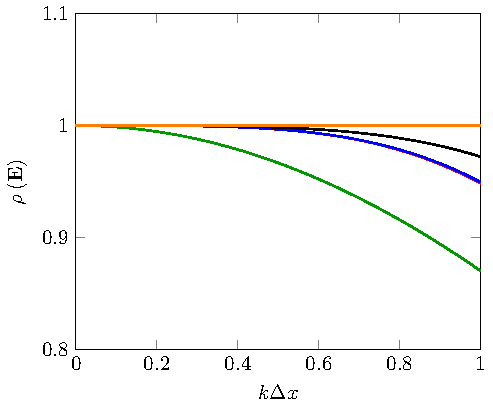
\includegraphics[width=\textwidth]{./chp5/figures/stabilityu=0kh0p5.pdf}
%		\subcaption*{\hspace{10 mm}$U =0$, $H = 1 $ and $k = 0.5$}
%	\end{subfigure}%
%	\begin{subfigure}{0.5\textwidth}
%		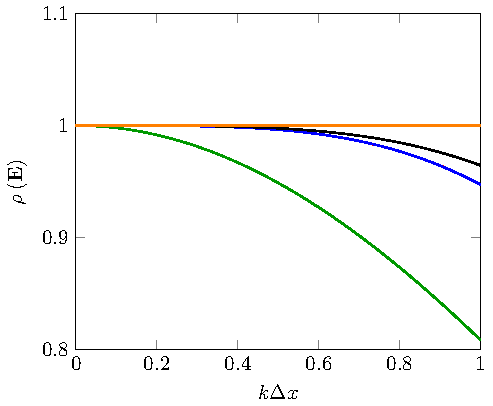
\includegraphics[width=\textwidth]{./chp5/figures/stabilityu=0kh2p5.pdf}
%		\subcaption*{\hspace{10 mm}$U =0$, $H = 1 $ and $k = 2.5$}
%	\end{subfigure}
%	\caption{Spectral radius of growth matrix $\matr{E}$ for first-order FDVM ({\color{green!60!black} \solidrule}), second-order FDVM({\color{red} \solidrule}), second-order FEVM ({\color{blue} \solidrule}), third-order FDVM ({\solidrule}), $\mathcal{D}$ ({\color{violet!80!white} \solidrule}) and $\mathcal{W}$ ({\color{orange} \solidrule}) .}
%	\label{fig:Stabu=0}
%\end{figure}
%
\begin{table}
	\centering
	\begin{tabular}{l  c  c}
		\hline
		Method & $kH$& Average\\
		\hline && \\
		$\mathcal{D}$& $0.5$ & $1+ 4\times 10^{-16}$  \\
		$\mathcal{D}$& $2.5$ & $1+ 4\times 10^{-16}$  \\
		\hline \\
		$\mathcal{W}$& $0.5$ & $1+ 4\times 10^{-16}$  \\
		$\mathcal{W}$& $2.5$ & $1+ 4\times 10^{-16}$ \\
		\hline
	\end{tabular}
	\caption{Average of $\rho\left(\matr{E}\right)$ over all $\Delta x$ values for the second-order finite difference methods when $U=0$.}
	\label{tab:Averageofspectralradiusu=0}
\end{table}
\subsubsection{Non-zero Mean Flow}
Only the finite difference methods $\mathcal{W}$ and $\mathcal{D}$ for the linearised Serre equations allow for nonzero values of $U$. We investigated the behaviour of the spectral radius of the growth matrix for various values of $U$, $kH$ and $\Delta x$. Again we have chosen $\Delta t =   \left( r / \left(U + \sqrt{gH}\right) \right) {\Delta x} $ with $r= 1/2$ to satisfy the CFL condition []. We present the results for $U =1$ with $kH =0.5$ and $2.5$ in Figure~\ref{fig:Stabu=1}. These values were chosen because they are representative of the behaviour for both methods for most values of $U$ and $kH$, and because these values of $kH$ match those used in the results above.

These results demonstrate that the naive second-order method $\mathcal{D}$ is still stable even with a background mean flow, with a spectral radius that is consistently $1$. This is demonstrated in Table~\ref{tab:Averageofspectralradiusu=1} as well where the average spectral radius is $1$ plus a number that is just round-off error. This behaviour was consistent for various $U$, $kH$ and $\Delta x$ values provided $0 < r \le 1$. Therefore this method is stable as desired for a range of flow scenarios. 

Unfortunately the finite difference/Lax-Wendroff method $\mathcal{W}$ is no longer stable anywhere with growth factors that are consistently larger than $1$ although it approaches stability as $\Delta x \rightarrow 0$. This is evident in Table \ref{tab:Averageofspectralradiusu=1} where the average spectral radius is larger than $1$ by significantly more than round-off error. By modifying the parameters we can increase the spectral radius of the evolution matrix for $\mathcal{W}$ as desired. The largest $k\Delta x$ value appears to correspond to our largest spectral radius. However, the interaction between the spectral radius, $hK$ and $U$ is not so obvious. Since the spectral radius was consistently larger than $1$ when $U \neq 0$ this means the Lax-Wendroff method is not stable unless $U=0$. Although the growth factors are only marginally greater than $1$ for most situations and so the instabilities may not be apparent when performing numerical experiments, as we demonstrate in Chapter []. 

We also investigated different relationships between $\Delta t$ and $\Delta x$, such as $\Delta t \propto \Delta x^a$ but could not find a reasonable $a$ that gave us stability for $\mathcal{W}$ when $|U| > 0$ across a range of $k\Delta x$ values.



\begin{table}
	\centering
	\begin{tabular}{l  c  c}
		\hline
		Method & $kH$& Average\\
		\hline && \\
		$\mathcal{D}$ & $0.5$ & $1+ 4\times 10^{-16}$  \\
		$\mathcal{D}$ & $2.5$ & $1+ 4\times 10^{-16}$  \\
		\hline \\
		$\mathcal{W}$ & $0.5$ & $1+ 6\times 10^{-3}$  \\
		$\mathcal{W}$ & $2.5$ & $1+ 3\times 10^{-3}$   \\
		\hline
	\end{tabular}
	\caption{Average of $\rho\left(\matr{E}\right)$ over all $\Delta x$ values for the second-order finite difference methods when $U=1$.}
	\label{tab:Averageofspectralradiusu=1}
\end{table}